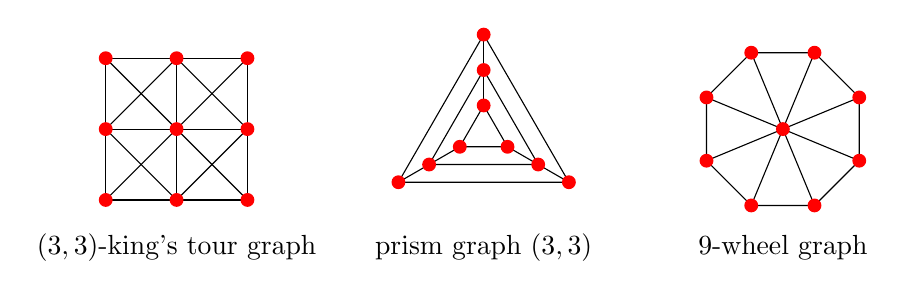
\begin{tikzpicture}[dot/.style={circle, fill=red, minimum size=5pt, inner sep=0pt}]
% (3,3)-king's tour graph: 3x3 grid, king moves (horizontal, vertical, diagonal)
\begin{scope}
  \foreach \i in {0,1,2} \foreach \j in {0,1,2} \coordinate (k\i\j) at (0.9*\i,0.9*\j);
  \foreach \i in {0,1,2} {\draw (k\i0) -- (k\i2); \draw (k0\i) -- (k2\i);}
  \foreach \i/\ii in {0/1,1/2} \foreach \j/\jj in {0/1,1/2} {\draw (k\i\j) -- (k\ii\jj); \draw (k\ii\j) -- (k\i\jj);}
  \foreach \i in {0,1,2} \foreach \j in {0,1,2} \node[dot] at (k\i\j) {};
  \node at (0.9,-0.6) {$(3,3)$-king's tour graph};
\end{scope}
% prism graph (3,3): three nested triangles joined along spokes
\begin{scope}[xshift=4.8cm, yshift=0.85cm]
  \foreach \r/\n in {1.25/o,0.8/m,0.35/i} \foreach \a/\k in {90/1,210/2,330/3} \coordinate (\n\k) at (\a:\r);
  \foreach \n in {o,m,i} \draw (\n1) -- (\n2) -- (\n3) -- cycle;
  \foreach \k in {1,2,3} \draw (o\k) -- (m\k) -- (i\k);
  \foreach \n in {o,m,i} \foreach \k in {1,2,3} \node[dot] at (\n\k) {};
  \node at (0,-1.45) {prism graph $(3,3)$};
\end{scope}
% 9-wheel graph: an octagon plus a hub joined to every vertex
\begin{scope}[xshift=8.6cm, yshift=0.9cm]
  \foreach \k in {0,...,7} \coordinate (w\k) at (22.5+45*\k:1.05);
  \draw (w0) \foreach \k in {1,...,7} {-- (w\k)} -- cycle;
  \foreach \k in {0,...,7} \draw (0,0) -- (w\k);
  \foreach \k in {0,...,7} \node[dot] at (w\k) {};
  \node[dot] at (0,0) {};
  \node at (0,-1.5) {$9$-wheel graph};
\end{scope}
\end{tikzpicture}
